
%(BEGIN_QUESTION)
% Copyright 2006, Tony R. Kuphaldt, released under the Creative Commons Attribution License (v 1.0)
% This means you may do almost anything with this work of mine, so long as you give me proper credit

Beregn verdiene i kalibreringstabellen under for en transmitter som måler væskegrensesnitt (spesifikke vekter = 0.8 og 1.0), med kalibreringstoleranse $\pm$ 1\% og utgangsområde 4-20 mA.  Angi hvilken port på $\Delta$P-transmitteren kalibreringstrykket skal påføres.

$$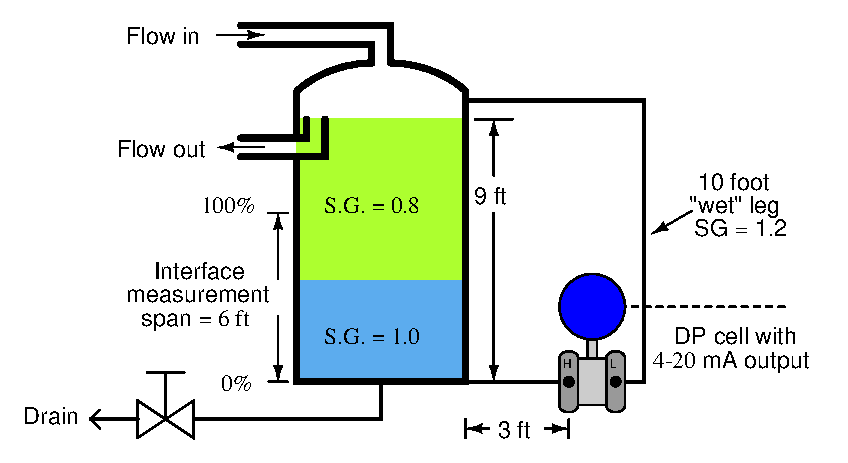
\includegraphics[width=15.5cm]{i00310x01.eps}$$

% No blank lines allowed between lines of an \halign structure!
% I use comments (%) instead, so that TeX doesn't choke.

$$\vbox{\offinterlineskip
\halign{\strut
\vrule \quad\hfil # \ \hfil & 
\vrule \quad\hfil # \ \hfil & 
\vrule \quad\hfil # \ \hfil & 
\vrule \quad\hfil # \ \hfil & 
\vrule \quad\hfil # \ \hfil & 
\vrule \quad\hfil # \ \hfil \vrule \cr
\noalign{\hrule}
%
% First row
Grensesnitt- & Prosent av & $\Delta$ trykk & Utgangssignal & Utgangssignal & Utgangssignal \cr
%
% Another row
nivå (ft) & spenn (\%) & målt ("W.C) & ideelt (mA) & min. (mA) & maks. (mA) \cr
%
\noalign{\hrule}
%
% Another row
  & 0 &  &  &  &  \cr
%
\noalign{\hrule}
%
% Another row
  & 10 &  &  &  &  \cr
%
\noalign{\hrule}
%
% Another row
  & 25 &  &  &  &  \cr
%
\noalign{\hrule}
%
% Another row
  & 50 &  &  &  &  \cr
%
\noalign{\hrule}
%
% Another row
  & 75 &  &  &  &  \cr
%
\noalign{\hrule}
%
% Another row
  & 90 &  &  &  &  \cr
%
\noalign{\hrule}
%
% Another row
  & 100 &  &  &  &  \cr
%
\noalign{\hrule}
} % End of \halign 
}$$ % End of \vbox

Vis all matematisk utregning slik at instruktøren kan kontrollere den konseptuelle gyldigheten av metoden(e) dine.  En god kontroll er å verifisere at alle mellomregninger har fysisk mening.  {\bf Hvis du virkelig forstår hva du gjør, vil du kunne identifisere riktig måleenhet for hvert mellomresultat og vise hvor tallet gjelder i scenariet}.

\vskip 20pt \vbox{\hrule \hbox{\strut \vrule{} {\bf Forslag til sokratisk diskusjon} \vrule} \hrule}

\begin{itemize}
\item{} Demonstrer hvordan man kan {\it estimere} numeriske svar uten kalkulator.
\item{} Hvordan vil transmitteren respondere hvis gasstrykket i tanken øker?
\item{} Hvordan vil transmitteren respondere hvis gasstrykket i tanken minker?
\item{} Hvordan vil transmitteren respondere hvis overløpsrøret blokkeres slik at lett væske ikke kan gå ut?
\item{} Hvordan vil transmitteren respondere hvis tettheten til den tyngre væsken øker, mens grensesnittnivået er uendret?
\item{} Hvordan vil transmitteren respondere hvis tettheten til den lettere væsken øker, mens grensesnittnivået er uendret?
\end{itemize}

\underbar{file i00310}
%(END_QUESTION)





%(BEGIN_ANSWER)

{\bf Delvis svar:}

% No blank lines allowed between lines of an \halign structure!
% I use comments (%) instead, so that TeX doesn't choke.

$$\vbox{\offinterlineskip
\halign{\strut
\vrule \quad\hfil # \ \hfil & 
\vrule \quad\hfil # \ \hfil & 
\vrule \quad\hfil # \ \hfil & 
\vrule \quad\hfil # \ \hfil & 
\vrule \quad\hfil # \ \hfil & 
\vrule \quad\hfil # \ \hfil \vrule \cr
\noalign{\hrule}
%
% First row
Grensesnitt- & Prosent av & $\Delta$ trykk & Utgangssignal & Utgangssignal & Utgangssignal \cr
%
% Another row
nivå (ft) & spenn (\%) & målt ("W.C) & ideelt (mA) & min. (mA) & maks. (mA) \cr
%
\noalign{\hrule}
%
% Another row
0 & 0 &  &  &  &  \cr
%
\noalign{\hrule}
%
% Another row
  & 10 &  &  &  & 5.76 \cr
%
\noalign{\hrule}
%
% Another row
  & 25 &  &  &  &  \cr
%
\noalign{\hrule}
%
% Another row
  & 50 &  & 12 &  &  \cr
%
\noalign{\hrule}
%
% Another row
4.5  & 75 &  &  &  &  \cr
%
\noalign{\hrule}
%
% Another row
  & 90 &  &  &  &  \cr
%
\noalign{\hrule}
%
% Another row
 & 100 & 43.2 (Low side) &  & 19.84 &  \cr
%
\noalign{\hrule}
} % End of \halign 
}$$ % End of \vbox

\vskip 10pt

Oppfølgingsspørsmål: hvorfor er det lurt å holde wet leg fylt med en væske med så høy spesifikk vekt (1.2)?  Hvorfor ikke la den fylles med den lettere væsken (SG = 0.8), eller bare vann (SG = 1.0)?

%(END_ANSWER)





%(BEGIN_NOTES)

\noindent
{\bf LRV-betingelse:}

Det er 9 fot lett væske mot transmitterens ``H''-port og 10 fot tung fyllvæske (SG = 1.2) mot ``L''-porten.  Differansetrykket ved LRV blir derfor:

$$\hbox{DP}_{LRV} = \left(9 \hbox{ ft} \over 1 \right) \left(12 \hbox{ in} \over 1 \hbox{ ft}\right) \left(0.8 \hbox{ in water} \over 1 \hbox{ in liquid} \right) - \left(10 \hbox{ ft} \over 1 \right) \left(12 \hbox{ in} \over 1 \hbox{ ft}\right) \left(1.2 \hbox{ in water} \over 1 \hbox{ in liquid} \right) $$

$$\hbox{DP}_{LRV} = (86.4 \hbox{ "WC}) - (144 \hbox{ "WC}) = -57.6 \hbox{ "WC}$$

\vskip 10pt

\noindent
{\bf URV-betingelse:}

Det er 6 fot vannlignende væske og 3 fot lett væske mot ``H''-porten, og 10 fot tung fyllvæske (SG = 1.2) mot ``L''-porten.  Differansetrykket ved URV blir derfor:

$$\hbox{DP}_{URV} = \left(6 \hbox{ ft} \over 1 \right) \left(12 \hbox{ in} \over 1 \hbox{ ft}\right) + \left(3 \hbox{ ft} \over 1 \right) \left(12 \hbox{ in} \over 1 \hbox{ ft}\right) \left(0.8 \hbox{ in water} \over 1 \hbox{ in liquid} \right) - \left(10 \hbox{ ft} \over 1 \right) \left(12 \hbox{ in} \over 1 \hbox{ ft}\right) \left(1.2 \hbox{ in water} \over 1 \hbox{ in liquid} \right) $$

$$\hbox{DP}_{URV} = (72 \hbox{ "WC}) + (28.8 \hbox{ "WC}) - (144 \hbox{ "WC}) = -43.2 \hbox{ "WC}$$

% No blank lines allowed between lines of an \halign structure!
% I use comments (%) instead, so that TeX doesn't choke.

$$\vbox{\offinterlineskip
\halign{\strut
\vrule \quad\hfil # \ \hfil & 
\vrule \quad\hfil # \ \hfil & 
\vrule \quad\hfil # \ \hfil & 
\vrule \quad\hfil # \ \hfil & 
\vrule \quad\hfil # \ \hfil & 
\vrule \quad\hfil # \ \hfil \vrule \cr
\noalign{\hrule}
%
% First row
Grensesnitt- & Prosent av & $\Delta$ trykk & Utgangssignal & Utgangssignal & Utgangssignal \cr
%
% Another row
nivå (ft) & spenn (\%) & målt ("W.C) & ideelt (mA) & min. (mA) & maks. (mA) \cr
%
\noalign{\hrule}
%
% Another row
0 & 0 & 57.6 (Low side) & 4 & 3.84 & 4.16 \cr
%
\noalign{\hrule}
%
% Another row
0.6 & 10 & 56.16 (Low side) & 5.6 & 5.44 & 5.76 \cr
%
\noalign{\hrule}
%
% Another row
1.5 & 25 & 54 (Low side) & 8 & 7.84 & 8.16 \cr
%
\noalign{\hrule}
%
% Another row
3 & 50 & 50.4 (Low side) & 12 & 11.84 & 12.16 \cr
%
\noalign{\hrule}
%
% Another row
4.5  & 75 & 46.8 (Low side) & 16 & 15.84 & 16.16 \cr
%
\noalign{\hrule}
%
% Another row
5.4 & 90 & 44.64 (Low side) & 18.4 & 18.24 & 18.56 \cr
%
\noalign{\hrule}
%
% Another row
6 & 100 & 43.2 (Low side) & 20 & 19.84 & 20.16 \cr
%
\noalign{\hrule}
} % End of \halign 
}$$ % End of \vbox

Det er lurt å holde wet leg fylt med en væske som er tyngre enn {\it alle} prosesskomponentene, i tilfelle grensesnittnivået stiger over toppen av wet leg.

\vskip 10pt

Merk at i denne situasjonen er ``low pressure''-siden av DP-cellen {\it alltid} utsatt for høyere absolutt trykk enn ``high pressure''-siden.  Dette virker paradoksalt til man husker at ``high'' og ``low'' ikke beskriver absolutt trykk, men {\it hvilken retning} hvert portbidrag påvirker transmitterutgangen i.  Et mer presist navnevalg kunne vært ``noninverting'' og ``inverting'', som på differensialforsterkere.

\vskip 10pt

Det horisontale 3-fotsmålet er overflødig informasjon, inkludert for å utfordre studentene til å vurdere om informasjonen er relevant for oppgaven.

%INDEX% Measurement, interface level: calibration table

%(END_NOTES)
